% !TEX root =../main.tex
\chapter{Estimador de estados}\label{chp-01}

\lettrine[lraise=-0.1, lines=2, loversize=0.2]{E}{n} muchas ocasiones se tienen sensores con un retraso y una frecuencia de actualización muy diferentes entre ellos, por ejemplo una IMU es mucho más rápida que el procesamiento de la imagen de una cámara. PX4 lo soluciona añadiendo más elementos a la estructura original de un estimador de estados. Uno de sus elementos es un \textit{Filtro de Kalman Extendido} (EKF). Este no usa las medidas más nuevas que le llegan, si no que las almacena y utiliza las que llegaron hace un determinado tiempo. Corriendo en paralelo pero a una frecuencia mayor, existe un estimador llamado \textit{Filtro de Salida}, el cual sí que utiliza la última medida del acelerómetro y del giróscopo. 

\section{Manejo de medidas retrasadas}
% TODO: Plantear los sensors y que da igual su periodos
% TODO: decir que el periodo de muestreo es de 5 ms

Supongamos que se tiene un sistema que se mueve en el espacio y del que se quiere conocer sus estados, en concreto, su posición, su velocidad y su orientación. Para este objetivo el sistema está dotado de numerosos sensores como que son un acelerómetro, un giróscopo, un barómetro, un GNSS o un sensor de flujo óptico. Cada uno de ellos tiene diferentes propiedades en cuanto a retraso, ruido, precisión, etc. Por ejemplo, la posición estimada por visión es una fuente muy precisa de posición, pero sin embargo tiene un gran retraso desde que se toma la imagen hasta que se procesa y se genera la medida. 

Para explicar un método de cómo afrontar  este problema, se va a poner un ejemplo de la ejecución paso a paso del estimador con diferentes sensores.
Supongamos que en el primera ejecución del estimador, se toma la primera medida de la IMU (acelerómetro y giróscopo). El EKF todavía no la utiliza, si no que la guarda en su buffer (figura \ref{fig:est1}). Conforme llegan nuevas medidas, que ocurre cada 5 ms, estas se introducen en la posición de más a la izquierda del buffer y las que ya estaban se van desplazando hacia la derecha, hasta que llegan a la última celda. La medidas de esta celda situada más a la derecha, son las que son usadas por el EKF. Los estados que este genera y las medidas utilizadas para estimarlos se refieren al \textit{horizonte de tiempo retrasado}. Como se muestra en la figura, el buffer tiene una longitud de 7 celdas, por lo tanto las medidas de la IMU que llegan al EKF siempre serán las que se recogieron hace 30 ms.  

\begin{figure}
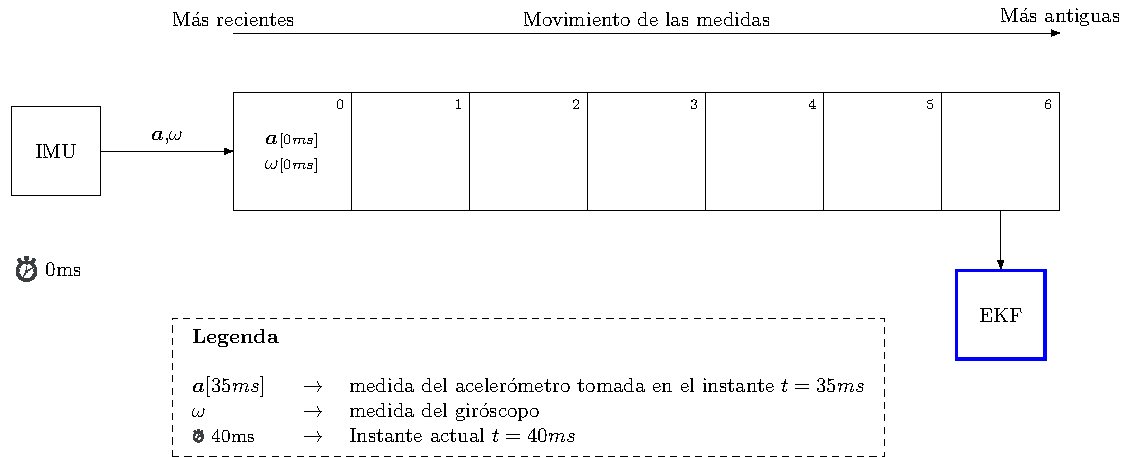
\includegraphics[width=\textwidth]{estimador_px4/tikz/ekf_output_1}
\caption{Primera medida tomada de la IMU}
\label{fig:est1}
\end{figure}

Pasan algunos ciclos más hasta que en el instante 50ms llega la primera medida del GPS, pero esta no se coloca en el extremo izquierdo del buffer junto con las medidas más recientes de la IMU, si no que se lleva directamente a la celda número 5 (ver figura \ref{fig:est2}). En esta también se encuentran las medidas de la IMU tomadas en el instante 25ms, es decir las que fueron tomadas hace 25 ms (50 ms -25 ms), que coincide con el retraso que tiene la posición del GPS con respecto a la IMU. De esta manera se agrupan las medidas que se refieren al mismo instante físico, es decir, el instante en el que llegaron pero {\bfseries compensándose su retraso}. 

\begin{figure}
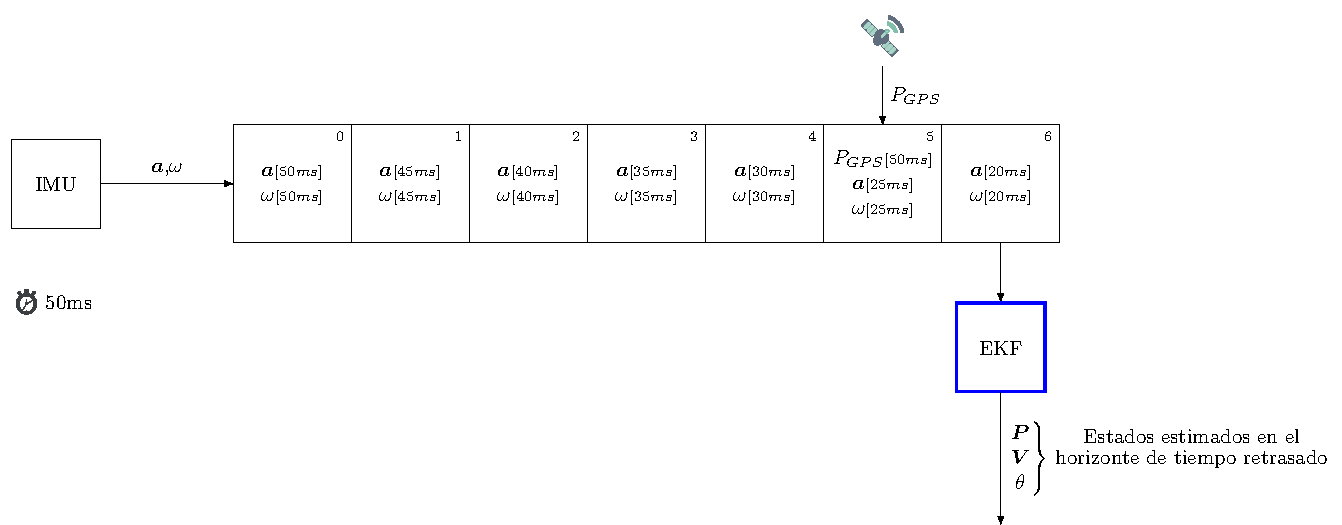
\includegraphics[width=\textwidth]{estimador_px4/tikz/ekf_output_2}
\caption{Llegada de la medida del GPS}
\label{fig:est2}
\end{figure}

De forma paralela se ejecuta el \textit{filtro de salida}, que es otro estimador de estados y para esta explicación se va a suponer que su funcionamiento interno es exactamente igual al del EKF, la única diferencia es que solamente utiliza las medidas de la IMU, en este caso las que se generan más recientemente. Estos estados se refieren al \textit{horizonte de tiempo actual} y son los únicos que se usan para las otras tareas que tenga vehículo, como por ejemplo para alimentar al controlador de orientación, por esta razón se le denomina filtro de salida. El problema que tiene este es que desaprovecha todos los demás sensores que tiene el vehículo, por lo que se le aplica un \textbf{mecanismo de corrección}.  

Este mecanismo está compuesto otro buffer llamado \textit{buffer de salida}, que se comporta de la misma manera que el primero, pero en lugar de guardar medidas, almacena los estados del filtro de salida. Estos estados se van desplazando hacia la derecha hasta que llegan a la última posición del buffer. En esta posición están los estados que se estimaron por el filtro de salida hace 30 ms, que coincide con el retraso que tienen las medidas del la IMU que entran al EKF. Si al EKF solo se le hubiese suministrado las medidas de la IMU, al igual que al filtro de salida, los estados del EKF y los que hay almacenado en esta última celda del buffer de salida coincidirían. Sin embargo, lo que está ocurriendo es que el EKF recoge medidas de otros sensores y por lo tanto no coincidirán. Para realizar la corrección, se calcula la diferencia entre ellos. Esta diferencia se atenúa y se le suma a todos los elementos del buffer de salida, además de al propio filtro de salida. 

% TODO: comentar otras medidas que han llegado

\begin{figure}
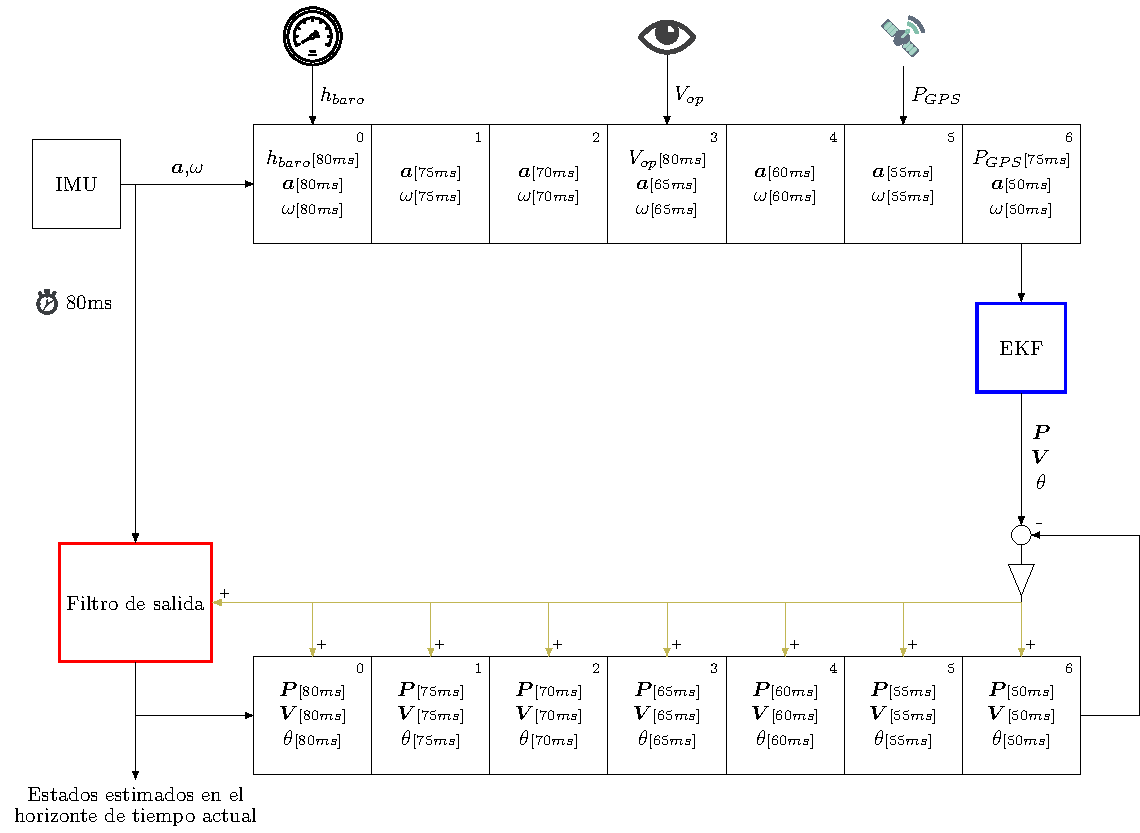
\includegraphics[width=\textwidth]{estimador_px4/tikz/ekf_output_3}
\caption{Estimador completo}
\label{fig:est3}
\end{figure}


{\color{red} [añadir detalles de implementación]}

\subsection{Detalles de implementación}
% tamaño de los buffer
En este apartado se presentan algunos trozos de código de PX4 que implementan lo anteriormente descrito más algunos detalles que he se han omitido en el apartado anterior para que fuese más fácil su comprensión.

En el apartado anterior se explicó que la error entre los estados estimados en el horizonte de tiempo retrasado y los estados del buffer de salida, se atenuaban (multiplicar por una ganancia menor que 1, mostrado en la figura \ref{fig:est3} como un triángulo) y se le suma a todo el buffer de salida. En el siguiente código se puede ver cómo se ha implentado esto. Se puede ver que la correción de la velocidad y la posición no solo se calcula a partir del error, sino también a partir de la integral del error, por lo tanto aqui se tiene un control proporcional-integral que tiene como señal de control la correción al buffer de salida. De esta manera, los estados en el horizonte de tiempo actual, se igualarán a los del horizonte de tiempo retrasado en régimen permanente. 

\begin{codigo}{Correción del buffer de salida. Ubicado en  la línea \href{https://github.com/PX4/PX4-ECL/blob/ec934908900b23ee273d1a9f82364b7b38423200/EKF/ekf.cpp\#L488}{488} del archivo \textit{Firmware/src/lib/ecl/EKF/ekf.cpp}}
\begin{minted}{c++}
void Ekf::applyCorrectionToOutputBuffer(float vel_gain, float pos_gain){
	// calculate velocity and position tracking errors
	const Vector3f vel_err(_state.vel - _output_sample_delayed.vel);
	const Vector3f pos_err(_state.pos - _output_sample_delayed.pos);

	_output_tracking_error(1) = vel_err.norm();
	_output_tracking_error(2) = pos_err.norm();

	// calculate a velocity correction that will be applied to the output state history
	_vel_err_integ += vel_err;
	const Vector3f vel_correction = vel_err * vel_gain + _vel_err_integ * sq(vel_gain) * 0.1f;

	// calculate a position correction that will be applied to the output state history
	_pos_err_integ += pos_err;
	const Vector3f pos_correction = pos_err * pos_gain + _pos_err_integ * sq(pos_gain) * 0.1f;

	// loop through the output filter state history and apply the corrections to the velocity and position states
	for (uint8_t index = 0; index < _output_buffer.get_length(); index++) {
		// a constant velocity correction is applied
		_output_buffer[index].vel += vel_correction;

		// a constant position correction is applied
		_output_buffer[index].pos += pos_correction;
	}

	// update output state to corrected values
	_output_new = _output_buffer.get_newest();
}
\end{minted}
\end{codigo} 

En el código anterior no ha aparecido la correción de la orientación, y esto es porque requieren que sea tratada a parte. En este estimador, la orientación se expresa en cuaternios y la operación de la correción no es simplemente una suma como ocurría en el caso de la velocidad, es más complicada y se tardaría demasiado en aplicarla a todos los elementos del buffer. En su lugar, únicamente se aplica una correción a la orientación estimada en el horizonte de tiempo actual.

\begin{codigo}{Correción de la orientación. Ubicado en el archivo \textit{Firmware/src/lib/ecl/EKF/ekf.cpp}}
En la línea \href{https://github.com/PX4/PX4-ECL/blob/ec934908900b23ee273d1a9f82364b7b38423200/EKF/ekf.cpp\#L323}{323} se corrige la orientación:
\begin{minted}{c++}
	// Apply corrections to the delta angle required to track the quaternion states at the EKF fusion time horizon
	const Vector3f delta_angle(imu.delta_ang - _state.delta_ang_bias * dt_scale_correction + _delta_angle_corr);
\end{minted}
En la línea \href{https://github.com/PX4/PX4-ECL/blob/ec934908900b23ee273d1a9f82364b7b38423200/EKF/ekf.cpp\#L411}{411} se calcula la ganancia del control
\begin{minted}{c++}
		// calculate a gain that provides tight tracking of the estimator attitude states and
		// adjust for changes in time delay to maintain consistent damping ratio of ~0.7
		const float time_delay = fmaxf((imu.time_us - _imu_sample_delayed.time_us) * 1e-6f, _dt_imu_avg);
		const float att_gain = 0.5f * _dt_imu_avg / time_delay;

		// calculate a corrrection to the delta angle
		// that will cause the INS to track the EKF quaternions
		_delta_angle_corr = delta_ang_error * att_gain;
\end{minted}
\end{codigo} 

%La ganancia que multiplica la diferencia entre el filtro de salida y el EKF y que sirve para corregir los estados, se calcula de manera el sistema controlado tenga un factor de amortiguamiento de 0.7.
%\begin{equation}
%K_p=\frac{0.5}{Retraso}
%\end{equation} 
%Puede que este valor se haya sacado de aproximar un retraso e^{sT} por un padé, como viene en https://www.researchgate.net/publication/237396133_RATIONAL_APPROXIMATION_OF_TIME_DELAY
% sin embargo no se como sacar el factor de amortiguamiento de funciones de tranferencia con ceros de fase no mínima.


\section{EKF para modelo bidimensional}
Se buscará un modelo discreto de espacio de estados descrito de la siguiente manera:
\begin{align}
X_{k+1} =  f(X_k)
\end{align}

Se va aplicar a un quadrotor en 2 dimensiones, pero el modelo al ser cinemático, se podría aplicar a cualquier otro móvil.

Estados:
\begin{align}
X = 
\begin{bmatrix} 
x \\ y \\ V_x \\ V_y \\ \theta
\end{bmatrix}
\end{align}

Modelo de predicción cinemático:
\begin{align}
\begin{bmatrix} 
x \\ y 
\end{bmatrix}_{k+1}
=
\begin{bmatrix} 
x \\ y 
\end{bmatrix}_k
+
\begin{bmatrix} 
V_x \\ V_y 
\end{bmatrix}_k
\Delta t
\end{align}

\begin{align}
\begin{bmatrix} 
V_x \\ V_y 
\end{bmatrix}_{k+1}
=
\begin{bmatrix} 
V_x \\ V_y 
\end{bmatrix}_k + 
\Delta t
\begin{bmatrix} 
\cos{\theta} & \sin{\theta} \\ -\sin{\theta} & \cos{\theta}
\end{bmatrix}
\bm{a} +  
\begin{bmatrix} 
0 \\ - m\ g 
\end{bmatrix}\Delta t
\end{align}

\begin{align}
\theta_{k+1} = \theta_k + \Delta t \omega
\end{align}


Jacobiano del modelo de predicción:
\begin{align}
F =\left. \frac{\partial f}{\partial X}\right| _{X_{k-1}} =  
\begin{bmatrix} 
%x/X
1 	&0	&\Delta t	&0		&0\\
%y/X
0 	&1	&0		&\Delta t	&0\\
%Vx/X
0 	&0	&1		&0		&\Delta t\left(-a_x\sin{\theta_{k-1}} + a_y\cos{\theta_{k-1}}\right) \\
%Vy/X
0 	&0	&0		&1		&\Delta t\left(-a_x\cos{\theta_{k-1}} - a_y\sin{\theta_{k-1}}\right) \\
%theta/X
0 	&0	&0		&0		&1
\end{bmatrix}
\end{align}

Jacobiano del acelerómetro y el giróscopo
\begin{align}
G =  \frac{\partial f}{\partial \bm{a},\omega} = 
\begin{bmatrix} 
%x/a,w
0 			&0			&0\\
%y/a,w
0 			&0			&0\\
%Vx/a,w
\Delta t \cos{\theta} 	&\Delta t \sin{\theta}	&0\\
%Vy/a,w
-\Delta t \sin{\theta} 	&\Delta t \cos{\theta}	&0\\
%theta/a,w
0 			&0			&\Delta t		
\end{bmatrix}
\end{align}

Matriz de covarianzas de la predicción:
\begin{align}
Q = 
G
\begin{bmatrix} 
\sigma^2_a 	& 0 		& 0\\
0 		& \sigma^2_a 	& 0\\
0 		& 0 		& \sigma^2_\omega\\
\end{bmatrix}
G^T
\end{align}

\section{Simulación del quadrotor y del estimador}
En este apartado se implementará el filtro explicado en este capítulo y pondrá a prueba con un simulador de un quadrotor. Tanto el estimador como el simulador estarán programados en lenguaje python. El simulador será muy sencillo, describirá el movimiento de un quadrotor en el plano al que únicamente se le aplican la fuerza de la gravedad, un empuje y un par. Estos dos últimos se serán generados por un controlador de velocidad vertical y un controlador de ángulo, los cuales toman la velocidad, y la inclinación real del vehículo en lugar de medidas ruidosas. Sus referencias se han escogido para que desde el reposo, ascienda unos metros, y luego se desplace hacia la dirección negativa del eje x. 


\begin{figure}
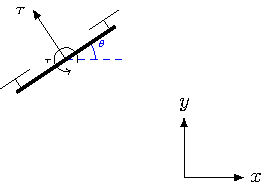
\includegraphics[width=0.5\textwidth]{estimador_px4/tikz/quadrotor_2d}
\caption{Quadrotor en dos dimensiones}
\label{fig:model}
\end{figure}

Para simular el quadrotor se realiza una integración discreta de la segunda ley de Newton:
\begin{align}
        \ddot{\theta} &= \frac{\tau}{I} \\
        \dot{\theta} &= \dot{\theta}_{i-1} + \Delta t \ddot{\theta} \\
        \theta &= \theta_{i-1} + \Delta t \dot{\theta} \\
        R &= 
\begin{bmatrix}
\cos{\theta}& -\sin{\theta}\\
\sin{\theta} & \cos{\theta}
\end{bmatrix}\\
         \bm{T_{rot}}&= R  \begin{bmatrix}0\\ T \end{bmatrix}\\
         \bm{F_g}&= \begin{bmatrix}0\\ -m g \end{bmatrix}\\
         \bm{a}& = \frac{\bm{T_rot}+\bm{F_g}}{m}\\
         \bm{v}& = v_{i-1} + \bm{a}\Delta t  \\
        \bm{p} &= p_{i-1} + \bm{v}\Delta t  \\
\end{align}


Una vez se ha simulado esta trayectoria, se pasa ejecutar el estimador de estados. Este toma unas medidas a las que se le ha aplicado un ruido gaussiano y genera su estimación de los estados. Finalmente estos se comparan con los estados reales y se verifica el desempeño del estimador. 

El primer experimento que se va a mostrar, al estimador de estados no le va a entrar ninguna otra medida que no sea la del giróscopo y la del acelerómetro (ver figura \ref{fig:simu1}) y en el segundo experimento (\ref{fig:simu2}) se va a fusionar la medida del GPS. Se puede ver que la fusión del GPS, aunque sea muy ruidosa, mejora en la estimación de la posición ya que no se produce la deriva del primer experimento. 

\begin{figure}
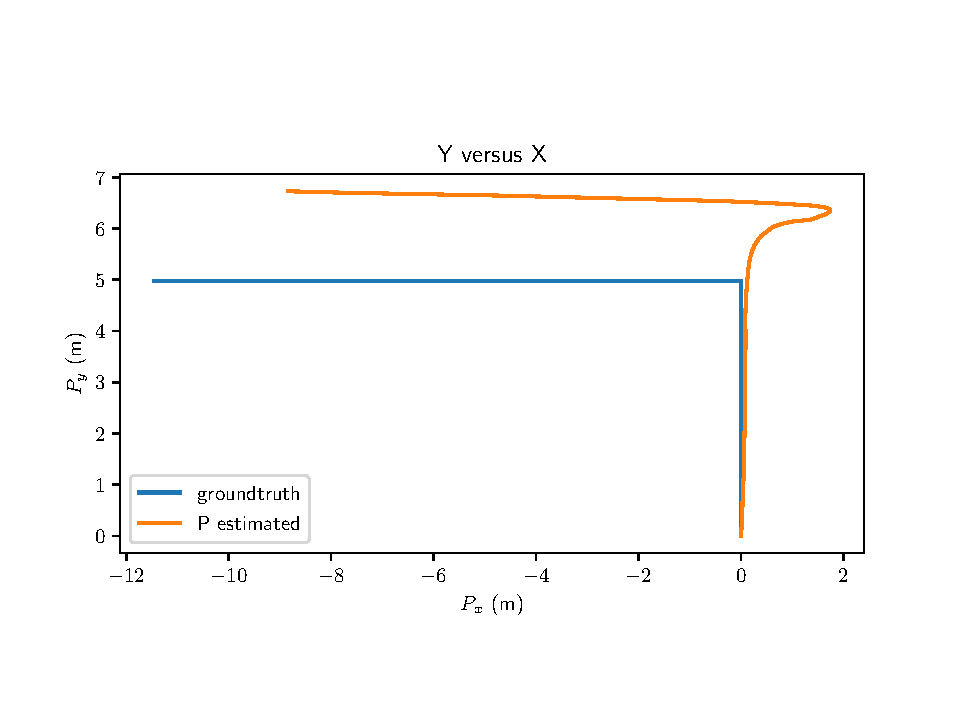
\includegraphics[width=\textwidth]{estimador_px4/im_simu/tray_no_gps}
\caption{EKF no ejecuta la fase de actualización}
\label{fig:simu1}
\end{figure}

\begin{figure}
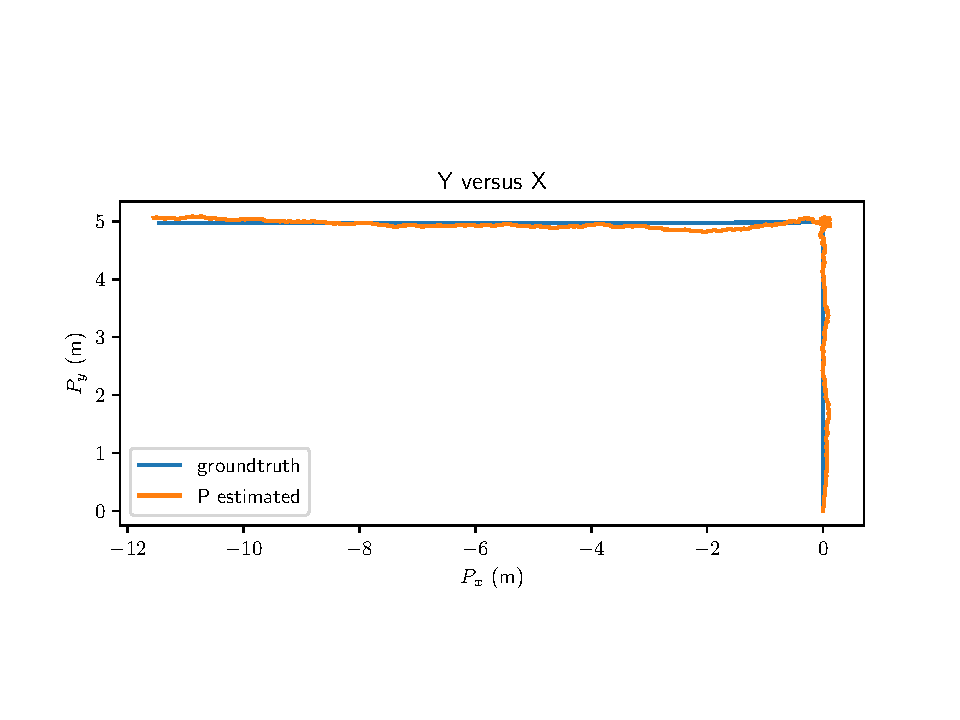
\includegraphics[width=\textwidth]{estimador_px4/im_simu/tray}
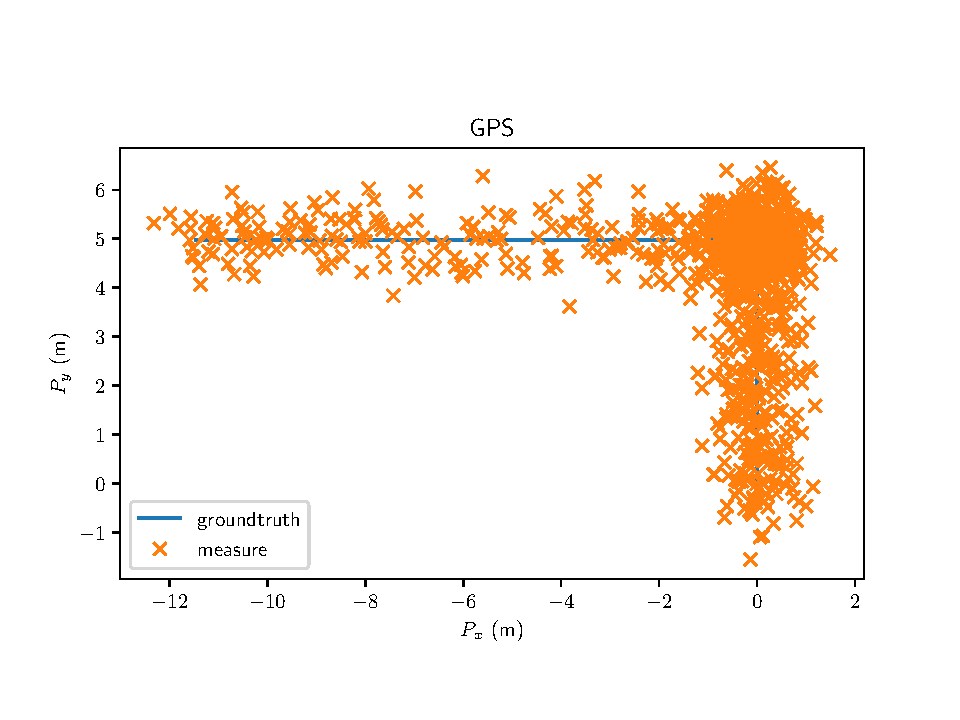
\includegraphics[width=\textwidth]{estimador_px4/im_simu/gps}
\caption{Fusionando la medida del GPS}
\label{fig:simu2}
\end{figure}


{\color{red} [Incluir GPS con retraso y comparar]}


{\color{red} [Incluir código explicado en anexo]}




\endinput
